\chapter*{Curriculum Vit\ae}
%\addcontentsline{toc}{chapter}{Curriculum Vit\ae}
%% Print the full name of the author.
% Profile picture, name and date and place of birth centered
\begin{center}
    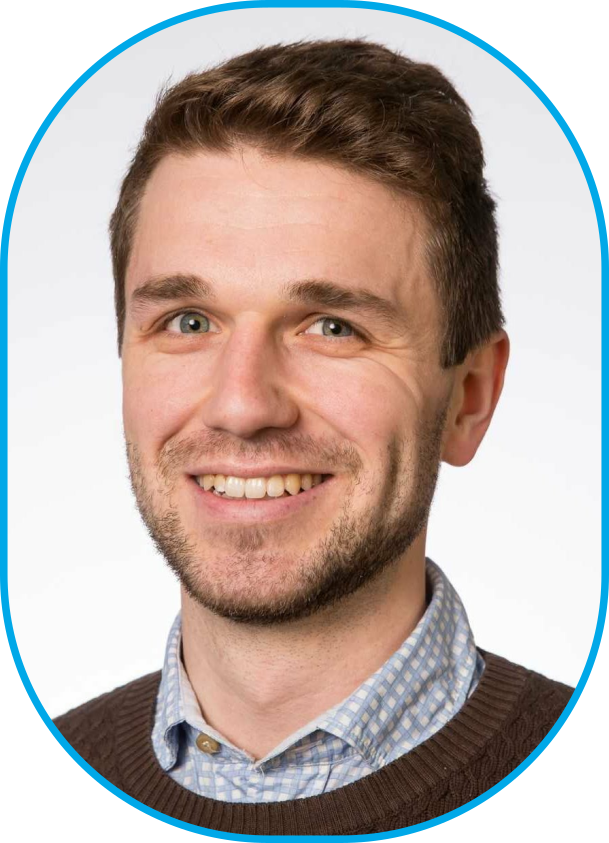
\includegraphics[width=0.3\textwidth]{src/helpers/cv/max_spahn.png}\\
    \vspace{0.5cm}
    {\Large\textbf{Max Spahn}} \\
    \vspace{0.2cm}
    \begin{tabular}{c}
        Born on 3 May 1994 in Bergisch Gladbach, Germany
    \end{tabular}
\end{center}

\section*{Education}

\begin{tabular}{p{0.15\linewidth} p{0.7\linewidth}}
  2013 & Abitur, Norbert Gynmasium, Dormagen, Germany\\
    2013--2019 & B.Sc. \& M.Sc. Mechanical Engineering, RWTH Aachen University, Germany\\
    2015--2017 & Diplôme d'ingénieur des Arts et Manufactures, École Centrale Paris, France\\
    2020--2024 & Ph.D. Robotics, Delft University of Technology, Netherlands \\
\end{tabular}

\section*{Robotic Competitions}
\begin{tabular}{p{0.15\linewidth} p{0.7\linewidth}}
  2022 & Winner ERF 2022 Franka Emika Hackathon Manipulation
  Challenge\\
  & \url{https://www.youtube.com/watch?v=eqpV09Kuc_o} \\
  2023 & Robothon 2023, Platonics Delft \\
  & \url{www.platonics.nl} \\
  2024 & Winner euROBIN Manipulation Skill Versatility Challenge at
  IROS, 2024, Platonics Delft \\
  & \url{www.platonics.nl} \\
\end{tabular}
